\documentclass[a4paper, openany]{memoir}

\usepackage[utf8]{inputenc}
\usepackage[T1]{fontenc} 
\usepackage[english]{babel}

\usepackage{fancyhdr}
\usepackage{float}

\usepackage{amsmath}
\usepackage{amsthm}
\usepackage{amssymb}
\usepackage{enumitem}
\usepackage{multicol}
\usepackage[bookmarksopen=true,bookmarksopenlevel=2]{hyperref}
\usepackage{tikz}
\usepackage{indentfirst}

\pagestyle{fancy}
\fancyhf{}
\fancyhead[LE]{\leftmark}
\fancyhead[RO]{\rightmark}
\fancyhead[RE, LO]{Data Fundamentals}
\fancyfoot[LE, RO]{\thepage}
\fancyfoot[RE, LO]{Pete Gautam}

\renewcommand{\headrulewidth}{1.5pt}

\chapterstyle{thatcher}
\setcounter{chapter}{5}
\begin{document}
\chapter{Time Series}
\section{Time series and signals}
Signals such as sound, light patterns and temperature are continuous in value and time/space. We can represent them as functions of time. We sample such functions with respect to time/space and represent them digitially. This involves quantising with respect to value and time/space. We have a precise set of values- $t$ and $x(t)$. Quantisation involves converting something into discrete set of values.

Let $x_t = x(t)$ represent a continuous (scalar) function with respect to time $t$. We sample it regularly to get a sequence of measurements $x[t] = [x_1, x_2, \dots, x_n]$. We do this by taking measurements at frequent, constant time intervals- the value $x(t)$ represents the value of the function at time $t$. This is time quantisation. The value $x(t)$ is further quantised so that it can be represented as fixed length in memory (e.g. to \texttt{float64}). This is amplitude quantisation. 

Following time and ampitude quantisation, we can convert a signal into a 1D array of data. Since we expect the measurements to be taken with the same time interval, we do not need to store time explicitly- we only need to specify/know the starting time (e.g. 1900 AD) and the sampling rate (e.g. every 10 years).

We call the 1D array of samples (without time values) the sampled signal. There is no value of $t$ stored- only the value $x(t)$; the time value is implied. Using the index of the value in the array, we can reconstruct the time value.

Along with the starting time, we need to store the sampling rate. This represents how frequently the data is being sampled. It is denoted by $f_s$. The unit of sampling is hertz (i.e. per second). In terms of spatial functions (e.g. images), the sampling rate is the number of measurements per some division of space (e.g. 72 pixels per inch). This value is also fixed when sampling, so we need not store the spatial coordinates in the sample.

We sample into signals to represent a continuous varying function in a compact, efficient manner. By not storing time, we are saving space. Also, since the data is represented as arrays, we can apply a vast collection of efficient/fast algorithms to them, in order to analyse the data. Some meaningful operations are:
\begin{itemize}
    \item removing an offset from a signal, which is equivalent to subtracting a value elementwise from a sample array.
    \item mixing two signals, which is equivalent to (weighted) elementwise sum of their sample arrays.
    \item correlation between signals, which can be computed using elementwise multiplication.
    \item selecting regions of signals, which can be done via slicing.
    \item smoothing and regression, which can be applied to signal arrays.
\end{itemize}

\subsection{Noise}
Whenever we measure signals, we will always have some noise. For some time $t$, there is some true value $y(t)$ and some noise $\epsilon(t)$- the value we measure is $x(t) = y(t) + \epsilon(t)$. The signal to noise ratio is given by
\[SNR = \frac{S}{N},\]
where $S$ the ampitude of $y(t)$ and $N$ is the ampitude of $\epsilon(t)$. A high $SNR$ means that the signal is quite clean and not corrupted with noise, while a low $SNR$ means that the signal is heavily corrupted (and weak). We can represent this logarithmically
\[SNR_{db} = 10 \log_{10} \left(\frac{S}{N}\right).\]
The units here is decibels. An increase of 10 decibels in the SNR makes the signal 10 times ``louder'' relative to the noise.

Ideally, we would want to remove all noise from the data. However, noise is random and difficult to control- it is therefore difficult to distinguish between noise and true data. However, if we make assumptions on the true value of the data $y(t)$, it is possible to remove some parts of the signal that couldn't be part of the true value. For example, the noise moving rapidly and we expect the true data to change at a much slower rate- we can remove/smoothen the values so that the dataset moves less rapidly. This is filtering- removing some parts of the data $x(t)$ based on our assumptions on $y(t)$. If our assumptions are wrong, we might lose the wrong data and fail to remove the noise.

\subsection{Sampling and noise}
Quantisation adds noise- the difference between the true value and the assigned value is random. There are different rates at which we could sample the data (i.e. time quantisation- converting continuous data to discrete samples; it makes the time $t$ discrete), and as the sampling rate increases, the noise decreases. Amplitude quantisation is how we realise this data into ndarrays- this makes the value $f(t)$ discrete. It reduces the range/precision of those values. There are typically a range of vels (or bits) that the value is represented as.

Amplitude quantisation introduces noise- there is a difference between the value of the signal $f(t)$ and the quantised level. With coarser quantisation, although we have more noise, we save storage space (and shorter time to perform computations on it). For example, we quantise a time signal below (from some audio) to 6 bits (i.e. $2^6 = 64$ levels).
\begin{figure}[H]
    \centering
    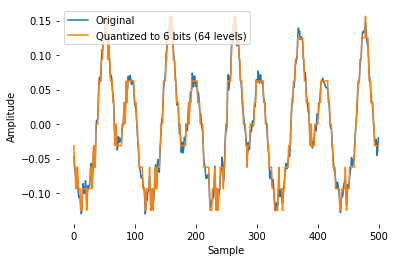
\includegraphics[scale=0.6]{src/6.1 quantised to 6 bits.png}
    \caption{Quantisation of a continuous signal into 6 bits.}
\end{figure}
\noindent We can also plot the residual difference.
\begin{figure}[H]
    \centering
    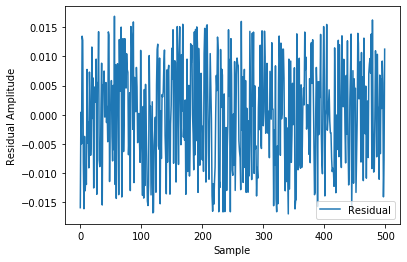
\includegraphics[scale=0.6]{src/6.2 residual amplitude.png}
    \caption{Residual amplitude of quantisation.}
\end{figure}
\noindent Clearly, the noise has no structure and is oscillating randomly.
\newpage

\section{Sampling theory}
If we sample a dataset enough, we can reconstruct a continuous signal perfectly, as long as that signal does not have too much high frequency content. In particular, Nyquist's limit tells us that for a sampling rate $f_s$, we can reconstruct the original signal from a sampled signal if the signal contains frequencies at most
\[f_n = \frac{f_s}{2}.\]
The value $f_n$ is called the Nyquist limit. For example, since human hearing extends to about 20 KHz, audio is often recorded with sample rate of 44.1 KHz.

If we do not sample enough (by not following this rule), the result is aliasing. In that case, when sampling a high-frequency $f_q > f_n$ (where $f_n$ is the sampling rate), we will observe an artificial component of $f_n - (f_q \bmod{f_n})$ in the sample (the value gets wrapped around). In videos, this creates a wagon wheel effect. Images must be filtered/smoothened to remove high-frequency components that cannot be sampled correctly before sampling (at a lower resolution)- this is called anti-aliasing. When the resolution of an image is reduced, the sample spacing gets larger, so the signal must have less high-frequency content if it is to be represented accurately.

\subsection{Regular sampling}
We must sample at regular intervals. Below we have a moving average line for the height and the volume of cherry trees. This data does not come from regular sampling, and is unordered.
\begin{figure}[H]
    \centering
    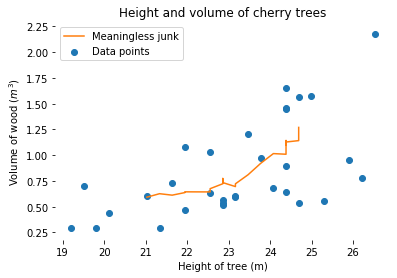
\includegraphics[scale=0.55]{src/6.3 height and volume of cherry trees.png}
    \caption{Height and volume of cherry trees, with a `line fit'.}
\end{figure}
\noindent So, the line isn't of much use (if any). The line isn't starting from the first component since the data is unordered. Instead, if we look at the number of air passengers oper year, the moving average behaves the way we want it to.
\begin{figure}[H]
    \centering
    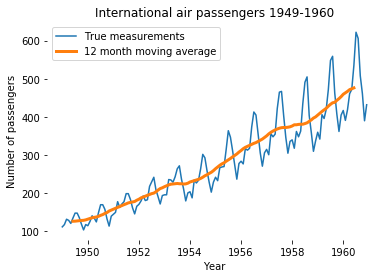
\includegraphics[scale=0.55]{src/6.4 international air passengers.png}
    \caption{International air passengers, with a line fit.}
\end{figure}
\noindent This is because the data was sampled at regular time intervals, and is ordered (with respect to time). 

So, we can only use the moving average if we have a regularly sampled signal. Nonetheless, there are 2 ways of drawing a line for cherry data. We can do regression (e.g. linear regression) to fit a line through the data (e.g. least squares), using optimisation or probability. We can also convert the data into regularly sampled form, and then use signal processing operations. This can be done using interpolation and resampling. This two-step process of interpolation and resampling is called gridding.

\subsection{Gridding}
The first step of gridding is interpolation- we estimate a value between some known measurements. An interpolating function produces estimates for a value of a function in between the data points. Let the data points be $[(t_0, x_0), \dots, (t_n, x_n)]$. Interpolation will give us a function $f$ such that $f(t_i) = x_i$ for all the data points. Moreover, the interpolated function $f$ can be evaluated anywhere between $x_0$ and $x_n$.

There are many ways to interpolate, such as:
\begin{itemize}
    \item constant/nearest neighbour interpolation- values are not changing between data points, i.e. we draw a straight line from the closest neighbour.
    \item linear interpolation- values are changing between data points in a linear way (a straight line between data points).
    \item polynomial interpolation- we fit a polynomial (typically quadratic or cubic) between data points.
\end{itemize}
Interpolations are most applied piecewise- we only care about the closest points before and after the point when interpolating. An example of interpolation is given below for the height and volume of cherry trees.
\begin{figure}[H]
    \centering
    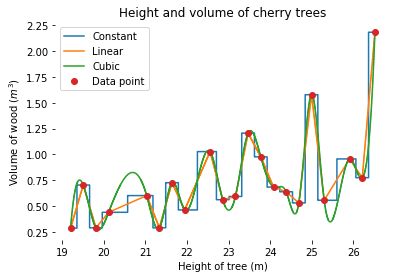
\includegraphics[scale=0.6]{src/6.5 height and volume of cherry trees with gridding.png}
    \caption{Height and volume of cherry trees, with several interpolations.}
\end{figure}
After interpolation, we resample. Using the interpolated graph, we evaluate $t$ at fixed time intervals to produce a time series. For the cherry trees example (with linear interpolation), we get the following moving average line:
\begin{figure}[H]
    \centering
    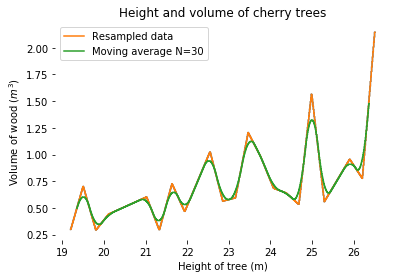
\includegraphics[scale=0.6]{src/6.6 height and volume of cherry trees with sampled.png}
    \caption{Height and volume of cherry trees, with a line fit using gridding.}
\end{figure}
We can use resampling to align multiple time series that are being sampled at different rates- we can resample to a common sampling rate. This alignment process is essential when combining sensor data from multiple streams.
\newpage

\section{Filtering and smoothing}
To remove noise from signals, we need to filter and smoothen it. Filtering takes advantage of the temporal structure of the data. We assume that the noise is random/independent. For example, we may have $x[t] = y[t] + \mathcal{N}(0, \sigma)$, where $y[t]$ is the true value and $\mathcal{N}(0, \sigma)$ is the noise. The values of $\sigma$ are independent with respect to time and the previous value $y[t-1]$.

One way of getting rid of noise is by averaging over multiple time steps. It will also average the true signal. But, we expect the true signal to not change fast- it will be similar to values around it. Moreover, the current value depends on the previous value. In particular, taking the average we won't damage the signal too much since the true value of the signal doesn't change fast.

\subsection{Moving average}
We expect the true signal to change slowly, but the noise to change fast and randomly. So, we can use a moving average to smoothen the signal. Here, for a given point, we take a sliding window around this point (we consider some points before and some after), and assign the value of this point to be the mean of all the values in the window. We iteratively compute all the values. Therefore, if $x[t]$ is the observed data with noise, the new data $y[t]$ is given by
\[y[t] = \frac{1}{K} \sum_{i=0}^{K-1} x[t+i-K/2].\]
The sliding window takes a smplied signal of some (maybe unbounded) length, and reduces it to a collection of fixed length vectors. We break the signal into equally spaced chunks/windows, each of length $K$. We then process these as an $N \times K$ matrix- $N$ windows of $K$ samples. We can perform any operations on these vectors/matrices (e.g. matrix operations, norms, quantisation). As we expect, the moving average depends on the length of the sliding window $K$- as $K$ gets bigger, the signal gets more smoothened out.

Using moving averages on sound reduces the high frequency content. The longer the moving average, the smoother the waveform and the more high-frequencies are suppressed. We can apply moving averages on images as well (spatially). This has the effect of blurring the image (box blur).
\newpage

\section{Nonlinear filtering}
Moving average is a linear filter- it is the weighted average. Linarity means: $f(x + y) = f(x) + f(y)$; $f(0) = 0$; $f(ax) = af(x)$.

\subsection{Median filtering}
Any filtering not using the weighted sum of the sliding window is a non-linear filter. An example of this is median filtering. This is like the moving average, but we use the median for each sliding window to decide on the value. This is applicable when most measurements are good, but few are corrupted with noise, especially if there is no guarantee that the noise is small.

This is a special type of order filter- in an order filter, we sort all the values in the sliding window before choosing a value. Other order filters take the minimum or the maximum, for example. 

Median filtering adds more robustness to extreme values than moving averages. The following image illustrates how linear and median filtering help remove noise from a corrupt signal.
\begin{figure}[H]
    \centering
    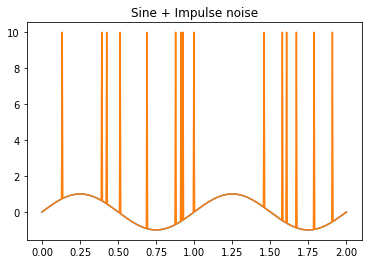
\includegraphics[scale=0.5]{src/6.8 sine with noise.png}
    \caption{The sine curve with impulsive noise.}
\end{figure}
\begin{figure}[H]
    \centering
    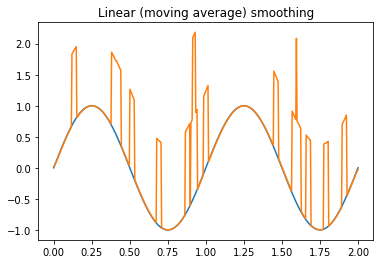
\includegraphics[scale=0.5]{src/6.9 sine with noise (linear).png}
    \caption{The sine curve with impulsive noise, smoothened by linear filtering.}
\end{figure}
\begin{figure}[H]
    \centering
    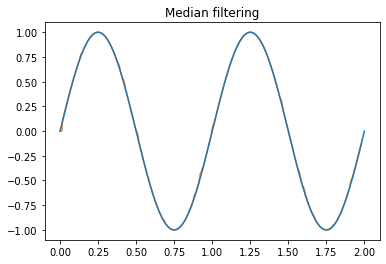
\includegraphics[scale=0.5]{src/6.10 sine with noise (median).png}
    \caption{The sine curve with impulsive noise, smoothened by median filtering.}
\end{figure}
\noindent Clearly, median filtering is much better at removing extrme outliers than linear filtering. However, since we need to sort the array/use specialised mean cascade algorithms, these algorithms are slower.
\newpage

\section{Convolution}
Most filters we apply are linear. These are very efficient and have been studied very well. A linear filter is a filter where the output is a weighted sum of the neighbouring values (and the original value). Although this is quite limited, there are many effects we can acheive using linear filtering. They are also quite efficient since the CPU (especially digital signal processing-specific CPUs) often have a multiply and accumulate operation. It can multiply by a constant and accumulate to a register. This makes linear filters very straightforward.

For example, a linear filter is
\[f(x[t]) = 0.25x[t-1] + 0.5x[t] + 0.25x[t+1].\]
This is a weighted sum of three sample. The total weight is still 1, so the average amplitude of the signal does not change. This filter has the effect of spreading a spike- it is a smoothening filter. The following illustrates this.
\begin{figure}[H]
    \centering
    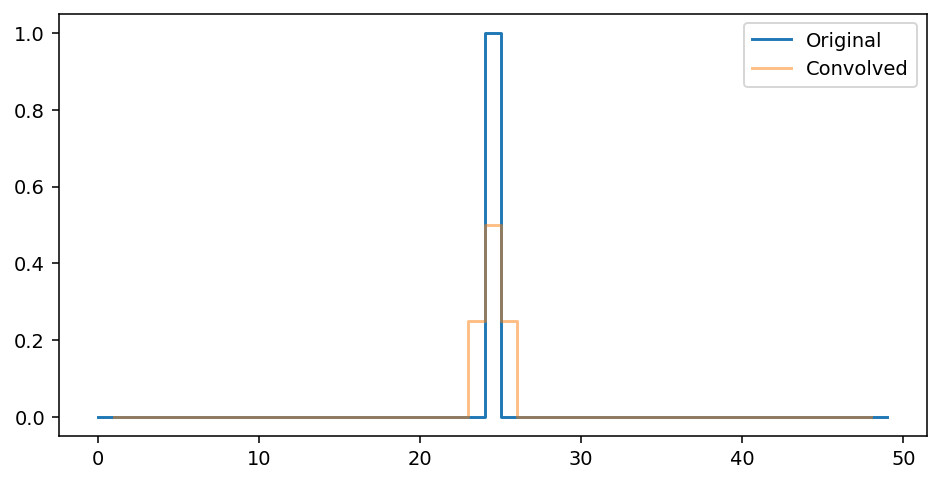
\includegraphics[scale=0.6]{src/6.11 convolved once.png}
    \caption{Applying a filter once to the signal.}
\end{figure}
\noindent We can keep applying this filter to the result, which keeps spreading and smoothening the spike.
\begin{figure}[H]
    \centering
    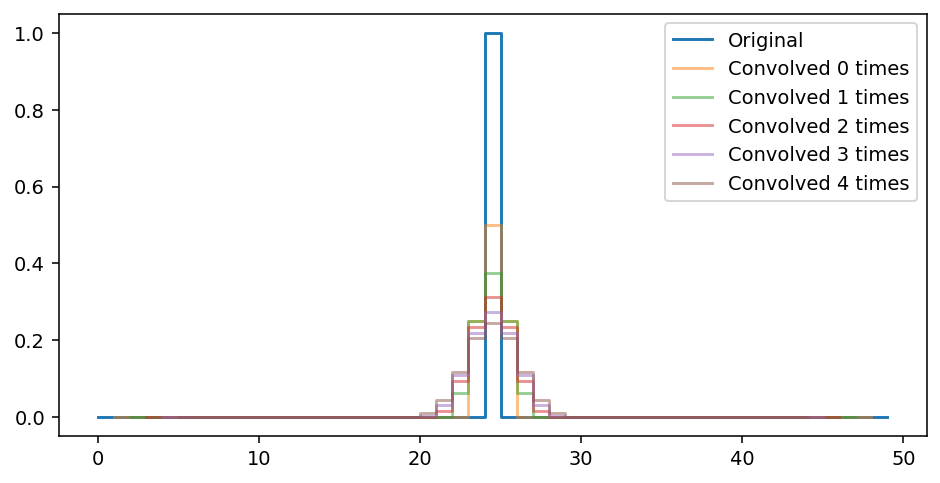
\includegraphics[scale=0.6]{src/6.12 convolved multiple.png}
    \caption{Applying a filter mutliple times to the signal.}
\end{figure}
\noindent The process of taking weighted sums of neighbouring values is called convolution.

For two functions $f$ and $g$, their convolution is denoted by $f * g$. Convolution is defined for continuous functions $f(x)$ and $g(x)$. For two sampled signal vectors $x[n], y[m]$ of length $N$ and $M$, the definition of convolution is
\[(x * y)[n] = \sum_{m=-M}^M x[n+m] y[m].\]
Note that we have $x[n+m]$ and not $x[m]$ since the sliding window starts at $x[n-M]$ and goes to $x[n+M]$. We can use convolution for effects like blurring and sharpening images, filtering audio, etc.

\subsection{The convolution kernel}
In $x * y$, we can think of $x$ as the signal to be transformed, and $y$ as the operation to be performed. We call $y$ the convolution kernel. It is an array, just like $x$. However, $x$ is normally much longer than $y$. For example, a convolution kernel is the array $[0.25, 0.5, 0.25]$. It has the following effect on the signals given.
\begin{figure}[H]
    \centering
    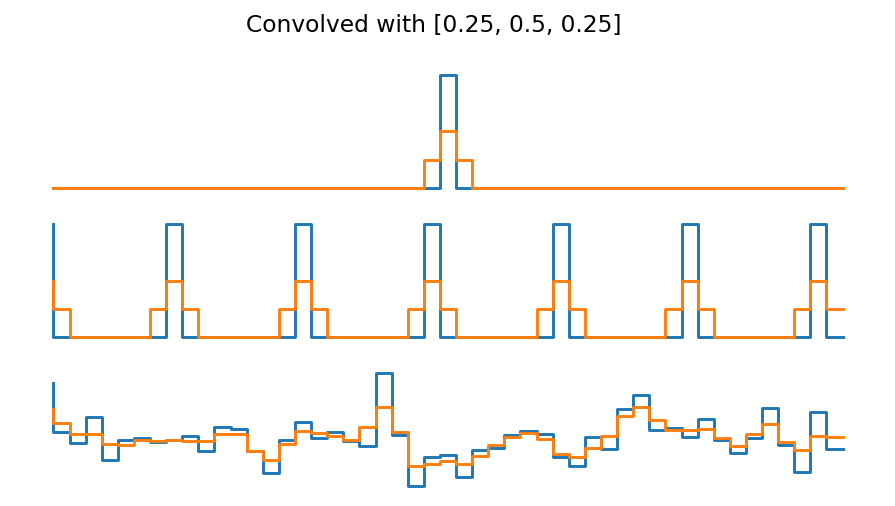
\includegraphics[scale=0.6]{src/6.13 convolved .25 .5 .25.png}
    \caption{Convolving signals with the convolution kernel $[0.25, 0.5, 0.25]$.}
\end{figure}

We can view moving average as a convolution- for example, if $N = 2$, then $y = [0.5, 0.5]$, and if $N = 5$, then $y = [0.2, 0.2, 0.2, 0.2, 0.2]$. The weighted sum of these values will give us the moving average. Each element in an array has the same value (equal weight), and they sum to 1 (no scaling of the amplitude).

\subsection{Algebraic properties of convolution}
The convolution operation is commutative, i.e. $f * g = g * f$, and associative, i.e. $(f * g) * h = f * (g * h)$. We can exploit the associativity property by first convolving the (much) short convolution kernels and then convolving with the time series, insteading of convolving with time series twice- we expect the signal to be much longer than the convolution kernels, so this will be much more efficient. Moreover, since the convolution operation is linear, it is distributive, i.e. $f * (g + h) = f * g + f * h$.

We illustrate these properties with an example. Consider the following convolutions- the edge detector convolution and the smoothing convolution. Their effects on the zero signal is given below.
\begin{figure}[H]
    \centering
    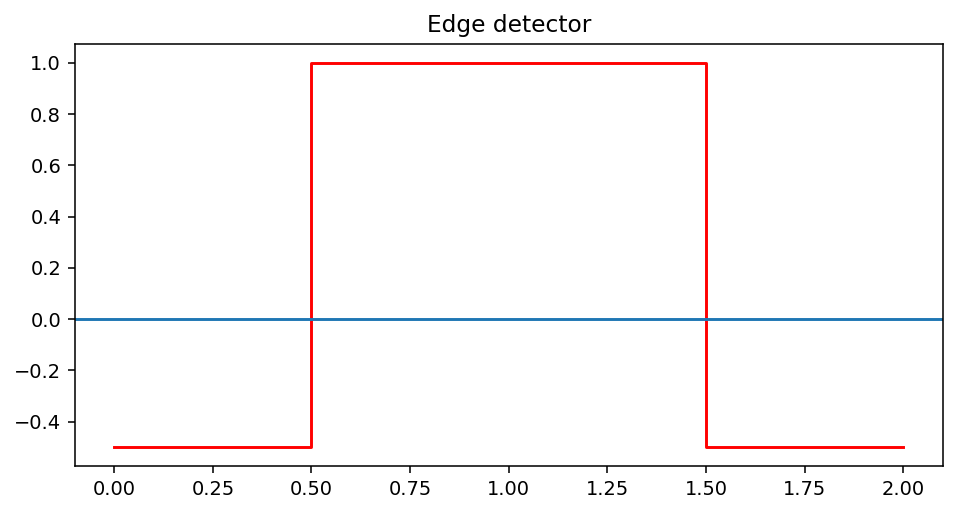
\includegraphics[scale=0.5]{src/6.14 edge detector.png}
    \caption{Applying the edge detector convolution kernel to the zero signal.}
\end{figure}
\begin{figure}[H]
    \centering
    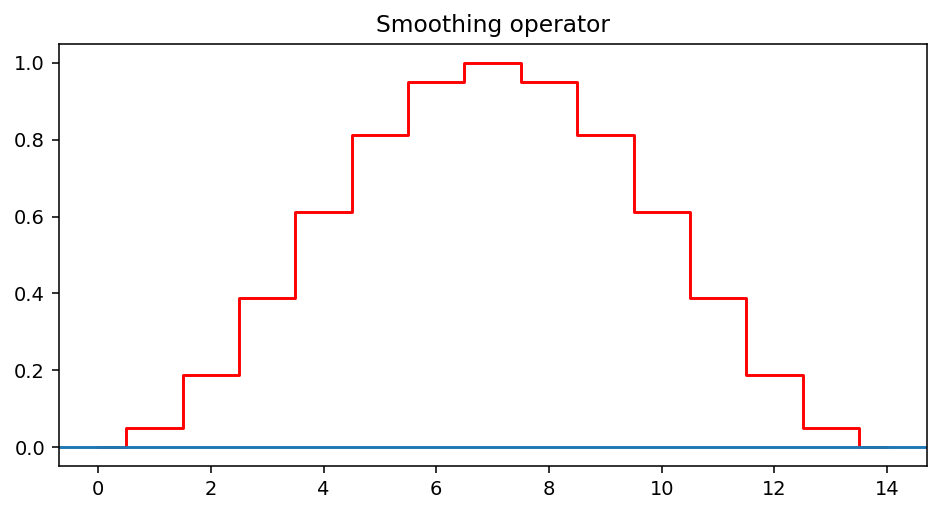
\includegraphics[scale=0.5]{src/6.15 smoothing operator.png}
    \caption{Applying the smoothing operator convolution kernel to the zero signal.}
\end{figure}
\noindent The convolving of these two kernels produces a smoothing edge detecting kernel. We will call it edgesmooth.
\begin{figure}[H]
    \centering
    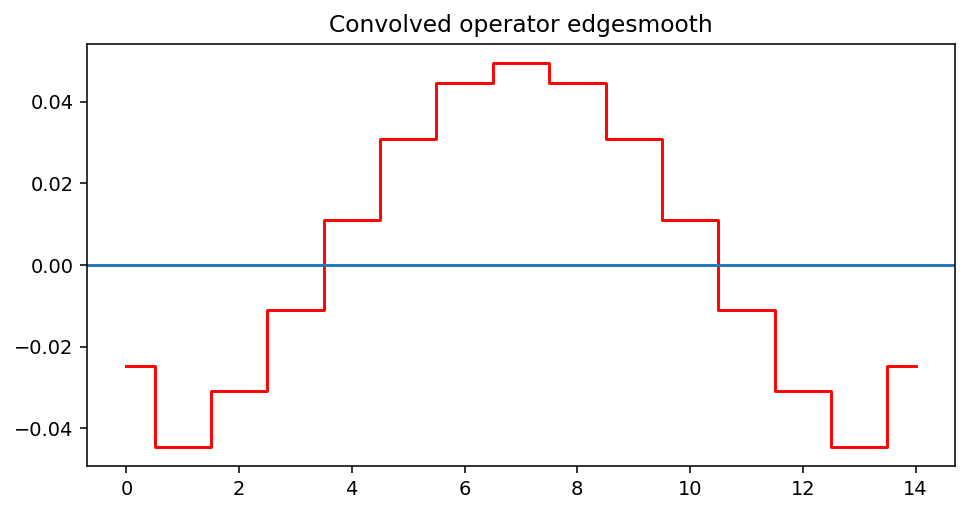
\includegraphics[scale=0.5]{src/6.16 edgesmooth.png}
    \caption{Applying the edgesmooth convolution kernel to the zero signal.}
\end{figure}
\noindent Now, consider a noisy saw signal.
\begin{figure}[H]
    \centering
    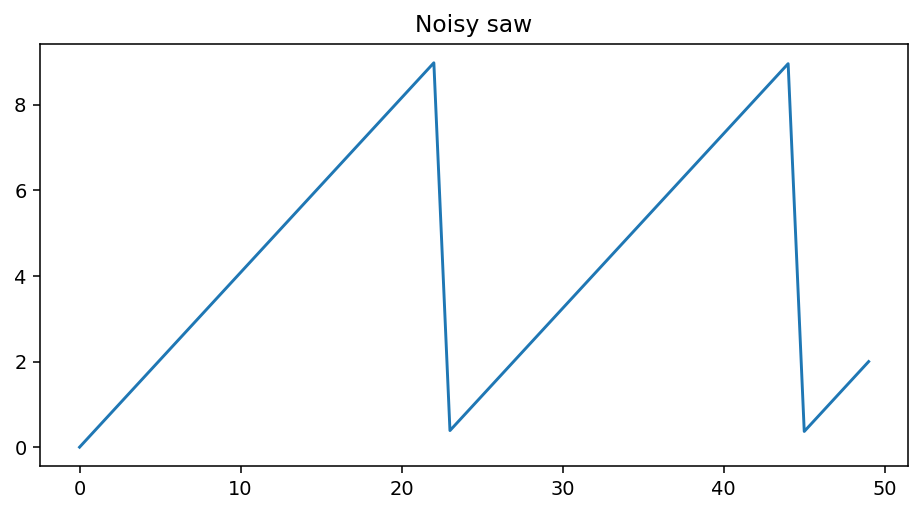
\includegraphics[scale=0.5]{src/6.17 noisy saw.png}
    \caption{A noisy saw signal.}
\end{figure}
\noindent If we apply the edge convolution to saw signal, and then the smoothing convolution, we get the following signal.
\begin{figure}[H]
    \centering
    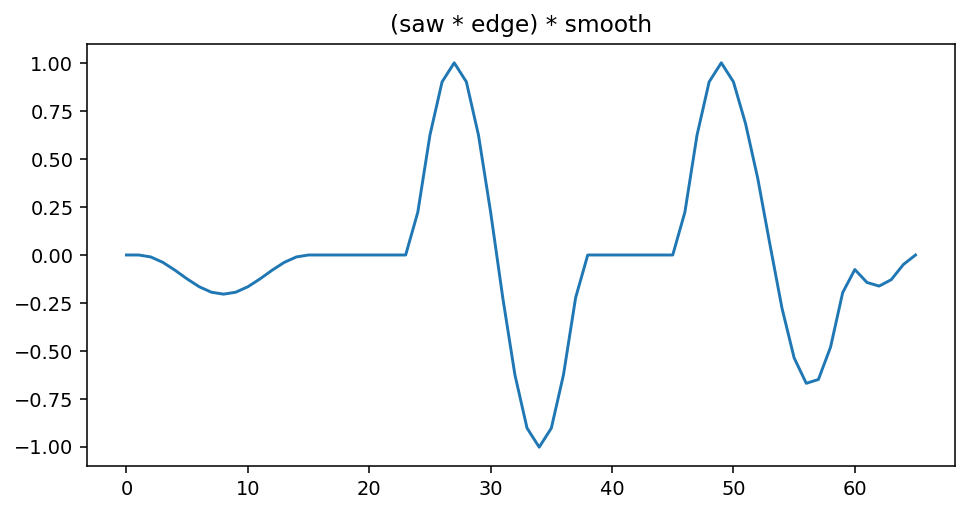
\includegraphics[scale=0.5]{src/6.18 saw, edge, smooth.png}
    \caption{Applying the edge convolution and then the smoothing convolution to the saw signal.}
\end{figure}
\noindent Moreover, if we apply the edgesmooth convolution to the saw signal, we get the following result:
\begin{figure}[H]
    \centering
    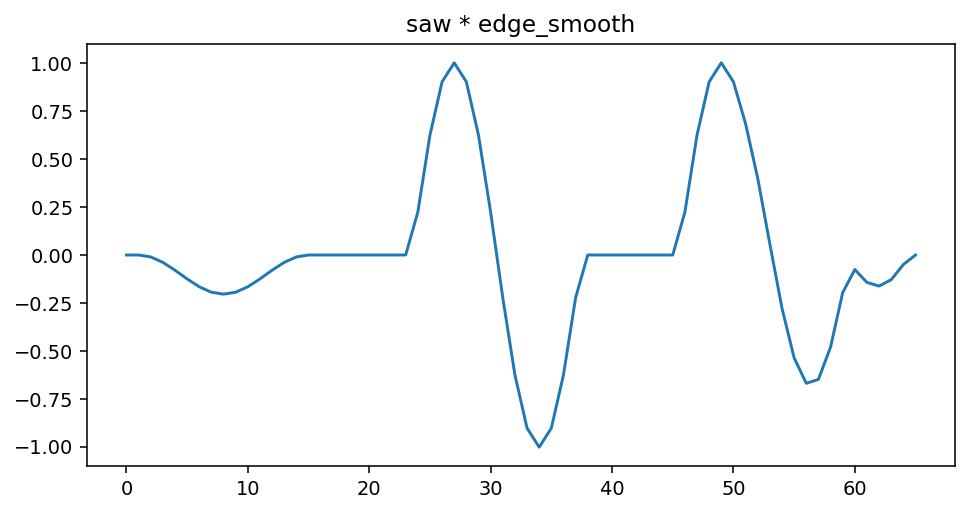
\includegraphics[scale=0.5]{src/6.19 saw, edgesmooth.png}
    \caption{Applying the edgesmooth convolution to the saw signal.}
\end{figure}
\noindent Clearly, they are the same. This illustrates the associativity of convolution.

\subsection{Dirac delta function}
The dirac delta function is given by
\[\delta(x) = \begin{cases}
    0 & x \neq 0 \\
    \infty & x = 0.
\end{cases}\]
This is not a proper function, but it satisfies
\[\int_{-\infty}^{\infty} \delta(x) \ dx = 1.\]

The delta function does not change other convolutions, i.e. $f * \delta = f$. It is an identity element with respect to convolution. Therefore, if we can simulate some system with the delta function, we can read back the convolution- it represents the linear model of the system.

The discrete version of the delta function is an array of zeroes with a single 1- the impulse. The figure below gives the discrete dirac delta function.
\begin{figure}[H]
    \centering
    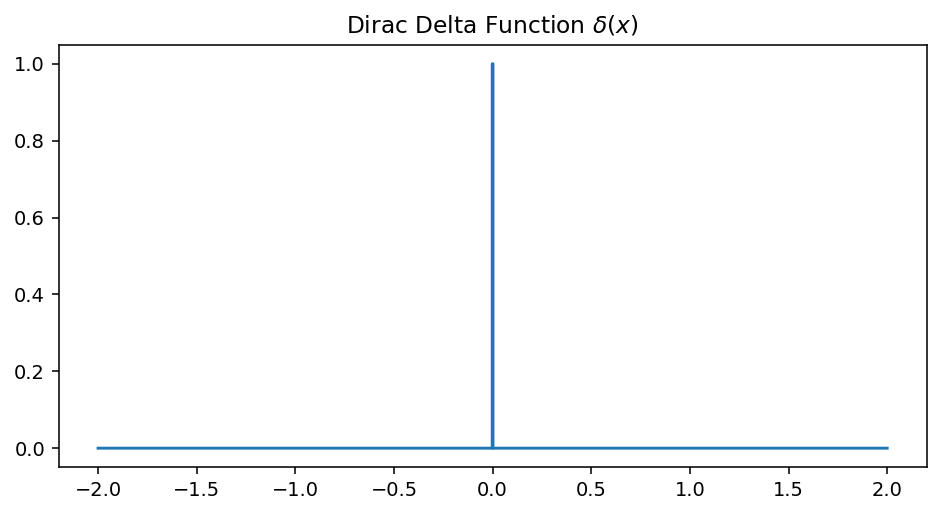
\includegraphics[scale=0.5]{src/6.20 dirac delta.png}
    \caption{The discrete dirac delta function.}
\end{figure}
\noindent If we feed a perfect impulse to the system, we can recover the convolution kernel. This is linear system identification.

% However, it is quite difficult to produce a perfect impulse in real world, as we need to deal with noise in the data. This is not an issue in the digital world as we can simulate noise-free impulses.
We can also use the delta function to capture something that behaves like a (linear) filter. We can inject the delta function to something so that we can create a filter representing this environment. Since the dirac delta function is the identity convolution, we can add to any signal to get the same sound back, but with this filter. In particular, we can add background feel to a sound (e.g. echo) using this property- this is called impulse response recovery, and is part of reverberation. Producing the dirac delta function (or any convolution) from the real world is difficult due to noise.
\newpage

\section{Frequency}
Until now, we have thought of a signal as a sequence of amplitude measurements over the time domain. We can also think of signals as a sum of oscillations over the frequency domain. These two representations are equivalent.

A pure oscillation is a sine wave
\[x(t) = A \sin (2 \pi \omega t + \theta),\]
where:
\begin{itemize}
    \item $\omega$ is the frequency of the oscillation;
    \item $\theta$ is the phase of the oscillation (offset to time); and
    \item $A$ is the magnitude (length of the amplitude) of oscillation.
\end{itemize}

A frequency is the repetition period of a sinusiodal oscillation. Higher frequency indicates a shorter period. The frequency domain representation represents signals as sums of oscillations at all frequencies, whre each frequency has a phase $\theta$ and magnitude $A$. A pure frequency is a sine wave with a specific period.

\subsection{Fourier transform}
The Fourier theorem tells us that any repeating function can be decomposed into sine waves. A single sine wave has a unique frequency $\omega$, amplitude $A$ and phase $\theta$, with $x(t) = A \sin (2\pi \omega t + \theta)$. The Fourier transform allows us to write any signal as a sum of sinusiod functions, i.e.
\[x(t) = \sum_i A_i \sin(2\pi \omega_i t + \theta_i).\]

To understand how the Fourier transform works, we can try to understand the correlation between signals $a[t]$ and $b[t]$. One way to do this is by computing the elementwise product of $a[t]$ and $b[t]$, for different values of $t$. When they are both the same sign, the product will be a large positive number; when they are opposite sign the product will be large negative number. We can sum the products
\[c = \sum_t a[t] b[t].\]
The value $c$ can be used to interpret the correlation between two signals, or the inner product representation of signals. If $c \approx 0$, then the two signals are not correlated. If $c$ is large and positive, then the two signals are similar, i.e. $a[t] = b[t]$. Instead, if $c$ is large and negative, the two signals are close to being inverse, i.e. $a[t] = -b[t]$.

If we now generate every possible frequency of sine wave as sampled signals $a_1[t], a_2[t], \dots$ and correlate each with a test signal $b[t]$, then for some $a[t]$, the result will be nearly zero (the signals are unrelated), while for others it will be larger (since $a[t]$ has some parts that are oscillating at the test frequency of $b[t]$). This is the amplitude $A$ of the response. Using this, we can compute the function $c(\omega)$, which is a sine wave and $c'(\omega)$ which is a cosine wave. Furthermore, we can compute the phase
\[\theta = \tan^{-1} \frac{c(\omega)}{c'(\omega)},\]
and the magnitude
\[A = \sqrt{c(\omega)^2 + c'(\omega)^2}.\]

The Fourier transform allows us to write any (periodic) function as an (infinite) sum of sinusoids. It gives simple waves with distinct frequencies, amplitudes and phases. The Fourier transform is defined as
\[\hat{f}(\omega) = \int_{-\infty}^{\infty} f(x) e^{-2\pi i \omega x} \ dx,\]
where
\[e^{2\pi i \theta} = \cos (2\pi \theta) + i \sin (2\pi \theta).\]
The result is a complex number, even for real-valued signals. The Fourier transform compares a function with every possible frequency of sine and cosine wave, and returns how much of that frequency is present and what phase the sinusoidal wave is in. The sine part and the cosine part are returned as the imaginary and the real components of this value respectively. The Fourier transform allows us to take transform a signal from the time domain to the frequency domain.

We can invert the Fourier transform to reconstruct the original function:
\[f(x) = \int_{-\infty}^{\infty} \hat{f}(x) e^{2\pi i x \omega} dx.\]
This is the inverse Fourier transform (IFT).

\subsection{Discrete Fourier transform}
For vector data $[x_0, \dots, x_{N-1}]$, the discrete Fourier transform (DFT) is given by
\[F[k] = \sum_{j=0}^{N-1} x[j] e^{-2\pi i \frac{j}{N}}.\]
The DFT has as many frequency components as $x[t]$ has elements.

Using the DFT, we can compute the phase $\theta$ and the magnitude $A$- this is the same as the angle and the magnitude of a complex number. The frequency of the component by the $k$ index depends on the sampling rate. $X_0 = 0$ and $X_{N/2} = f_n$, where $f_n$ is the Nyquist rate (half the original sampling rate). So, for the $k$-th component, the real frequency in terms of the original signal is: $\operatorname{freq} = f_n k/N$. This gives us an amplitude and phase for each component between 0 and $f_N$ in evenly spaced subdivisions, with as many subdivisions as there were elements of $x[t]$.

We illustrate this with some examples. Consider the following signal generated by the sum of 2 sine curves.
\begin{figure}[H]
    \centering
    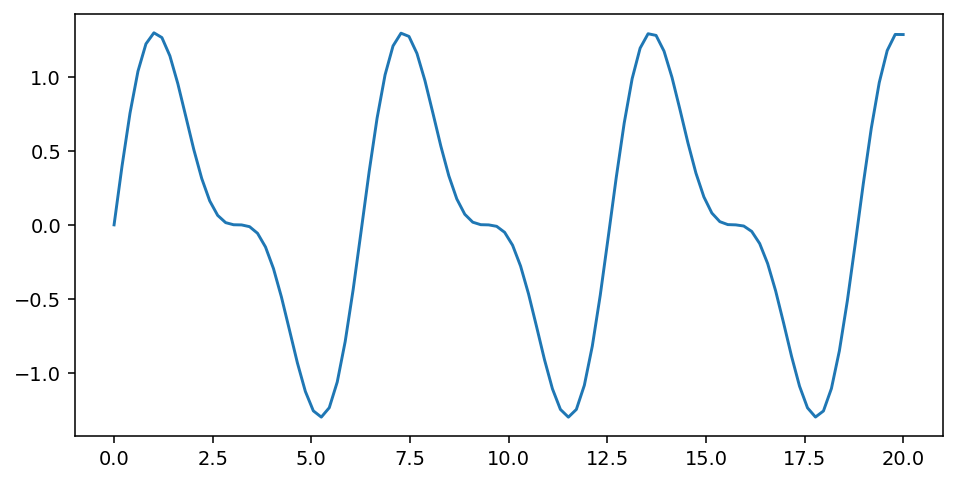
\includegraphics[scale=0.5]{src/6.21 sine curves.png}
    \caption{A signal created by 2 sine curves.}
\end{figure}
The DFT of this signal is the following.
\begin{figure}[H]
    \centering
    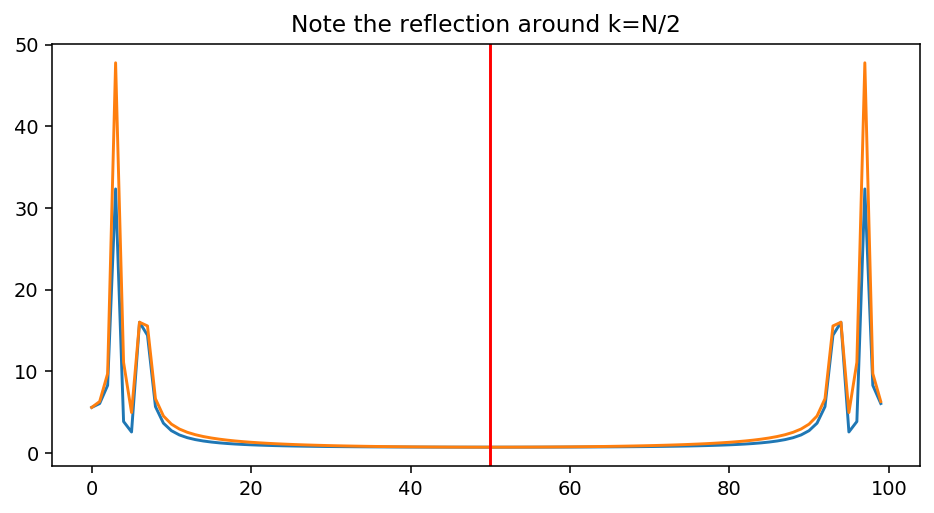
\includegraphics[scale=0.5]{src/6.22 sine curves dft.png}
    \caption{The DFT of the signal above.}
\end{figure}
\noindent We can see 2 frequency bands in the DFT, for the two different frequencies in the signal. The DFT is symmetric around $k = \frac{N}{2}$, and arises by the definition of the Fourier transform. In the following example, we have a single sine curve with frequency 440 Hz.
\begin{figure}[H]
    \centering
    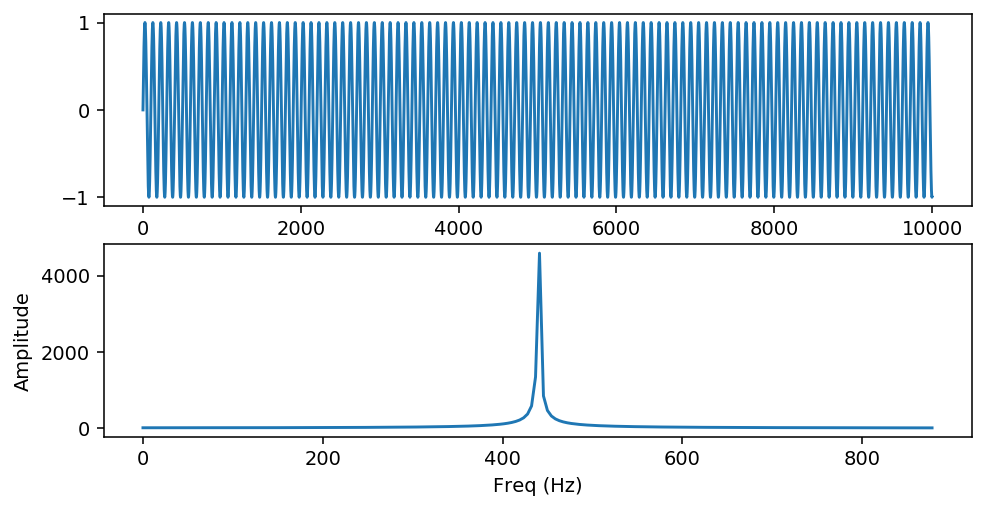
\includegraphics[scale=0.5]{src/6.23 sine to DFT frequency.png}
    \caption{The DFT of the signal above.}
\end{figure}
\noindent We can extract the frequency/ampitude directly from the DFT. Moreover, if we have 15 sinusiods in our signal, the DFT can give us back the frequency/ampitude of each of them.
\begin{figure}[H]
    \centering
    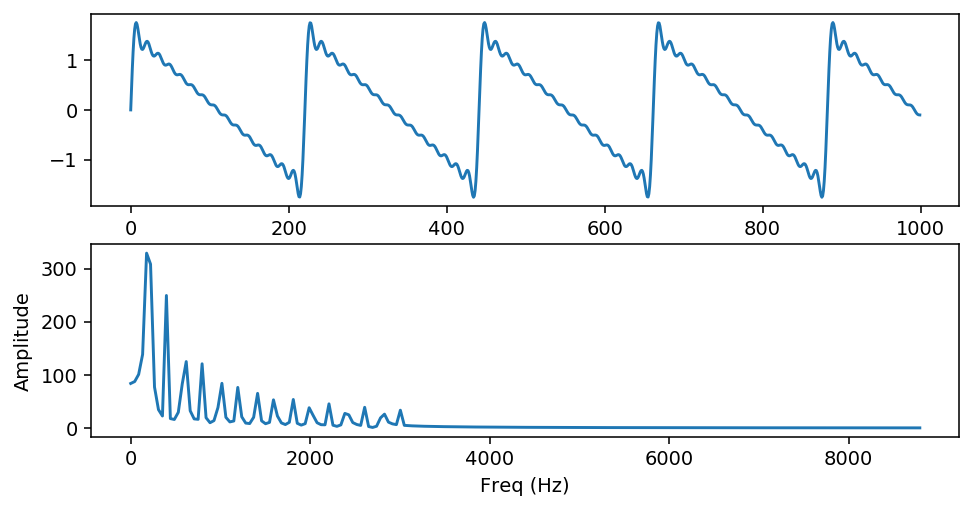
\includegraphics[scale=0.5]{src/6.24 15 sine curves fourier.png}
    \caption{The DFT of a signal composed of 15 sine curves.}
\end{figure}
\noindent Using this result, we can reconstruct the original signal (using the inverse DFT), but with only the first few frequencies. We typically choose those with the highest amplitude since they affect the signal the most.
% We can perform the Fourier transform, decompose into components, and then reconstruct with the $k$ most important (loudest) frequency components.

The naive implementation of DFT is $O(N^2)$, with lots of expensive floating point oprations like exponentiation. There is a fast Fourier transform (FFT), which is $O(N \log N)$ and uses divide-and-conquer strategy. The FFT is $O(N \log N)$ if $N$ is a power of two (because the standard FFT splits the signal recursively into two), and $O(N^2)$ for any other number. Variations of FFT run in $O(N \log N)$ for vectors with length which is highly composite, but still $O(N^2)$ for prime $N$.

\subsection{The convolution theorem}
The convolution theorem states that the Fourier transform of the convolution of two signals is equal to the (elementwise) product of the Fourier transform of the two signals. That is,
\[FT(f(x) * g(x)) = FT(f(x)) \cdot FT(g(x)),\]
where $*$ is convolution and $\cdot$ is elementwise product. Using this identity, we can compute the convolution $f * g$ by
\[f(x) * g(x) = IFT(FT(f(x)) \cdot FT(g(x))).\]
In particular, we can compute the convolution in $O(N \log N)$ time.

\subsection{Frequency domain effects}
Time domain convolution affects the frequency spatial domain, as we can see in the convolution theorem. We can use this to analyse the effects of filters before we apply them to images. We can apply any frequency-based filter in the frequency domain by simply multiplying; but having to take the DFT can be much slowr and much more memory intensive than a small convolution. The opposite is true for large convolutions.

The following are some types of filters:
\begin{itemize}
    \item a smoothing/lowpass filter- reduces high frequencies;
    \item a highpass filter- reduces low frequencies;
    \item a bandpass filter- reduces frequencies out of a certain band; and
    \item a notch/bandstop filter- reduces frequencies inside a certain band.
\end{itemize}

A linear filter (i.e. a convolution) can change the amplitude of frequencies, but not introduce a new one. If a frequency is not present in a signal, no linear filter can make it appear. Only non-linear filters can introduce new frequencies. This follows from the convolution theorem- since
\[FT(f(x) * g(x)) = FT(f(x)) \cdot FT(g(x)),\]
no matter what $g(x)$ is, if $FT(f(x)) = 0$ (i.e. no frequency present), then the convolution will also have $FT(f(x) * g(x)) = 0$.

\subsection{Sunspots example}
We can apply some filters to the sunspots data- the number of sunspots seen every 5 years.
\begin{figure}[H]
    \centering
    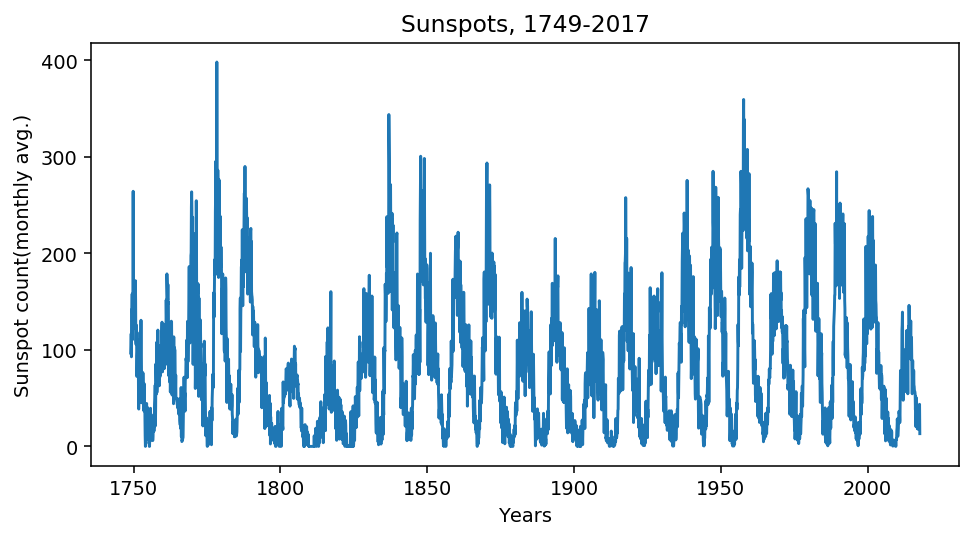
\includegraphics[scale=0.6]{src/6.25 sunspots original.png}
    \caption{The number of sunspots seen every 5 years.}
\end{figure}
\noindent We can apply the DFT (along with a smoothening filter) to extract the frequencies of the signal.
\begin{figure}[H]
    \centering
    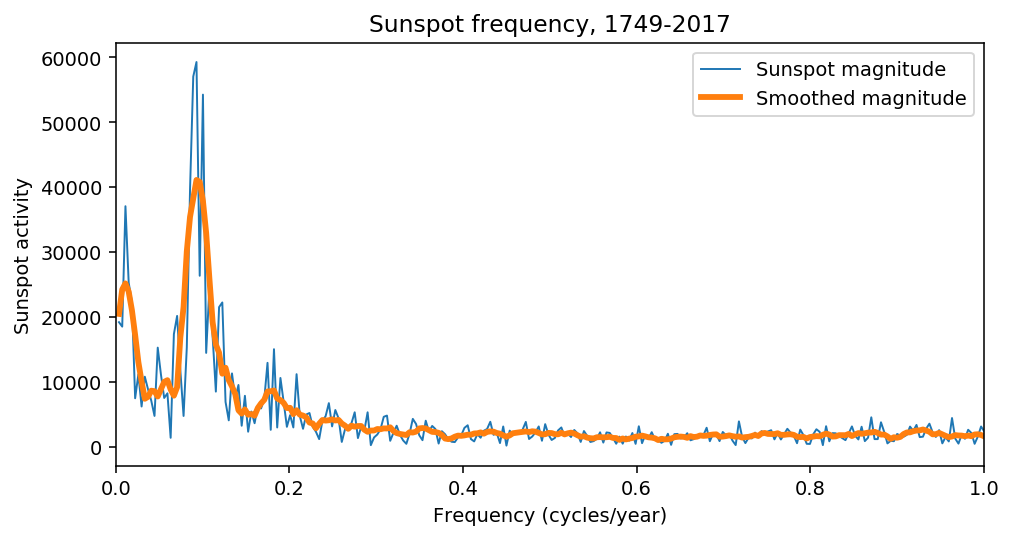
\includegraphics[scale=0.6]{src/6.26 sunspots smooth.png}
    \caption{The frequency of sunspots seen every 5 years constructed by the DFT, with a smoothening filter.}
\end{figure}
\noindent This data can be thought of as having 3 components:
\begin{itemize}
    \item random fluctuations, which vary from day to day, which would be a high frequency noise;
    \item some long term trend (e.g. the sun rotating around the galaxy), which would be a low-frequency oscillation; and 
    \item the oscillation of the nuclear processes within the sun.
\end{itemize}
\noindent This can be seen in the image below.
\begin{figure}[H]
    \centering
    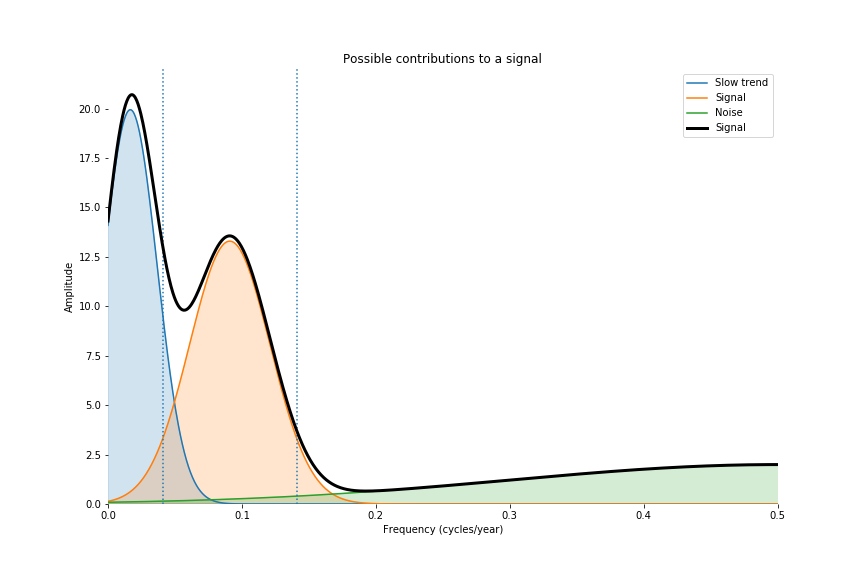
\includegraphics[scale=0.35]{src/6.27 3 components.png}
    \caption{Possible contribution to the signal.}
\end{figure}
\noindent These 3 components produce 3 different fequencies. In this case, there is some kind of peak around about 0.1 cycles/year, or every 10 years. This is visible on the magnitude spectrum plot. By the convolution theorem, we can design a filter to select only these frequencies. We just define a mask in frequency space, convert to the time domain using the IFT and convolve. We can also multiply in the frequency domain and then invert- this is the same according to the convolution theorem.

So, we will create a simple function in the frequency domain that will select the frequencies we are interested in, and mask out the remainder. A Gaussian function (used for the PDF of a normal distribution) is an effective mask to use, as it is nice and smooth. We will use the one centered at 0.1.
\begin{figure}[H]
    \centering
    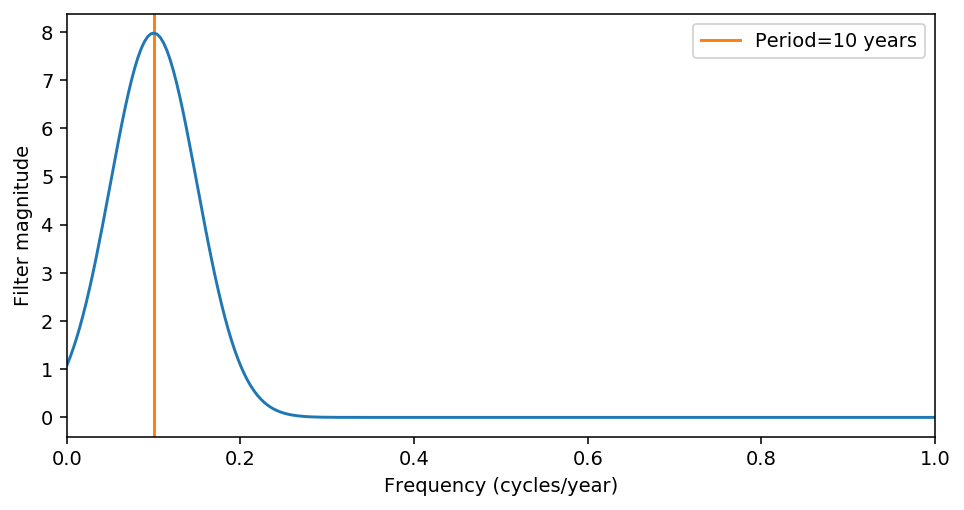
\includegraphics[scale=0.6]{src/6.28 chosen frequency.png}
    \caption{The chosen filter.}
\end{figure}
\noindent We can now take this frequency domain representation, and convert it to the time domain using the IFT. This will give us a convolution kernel we can apply to the signal.
\begin{figure}[H]
    \centering
    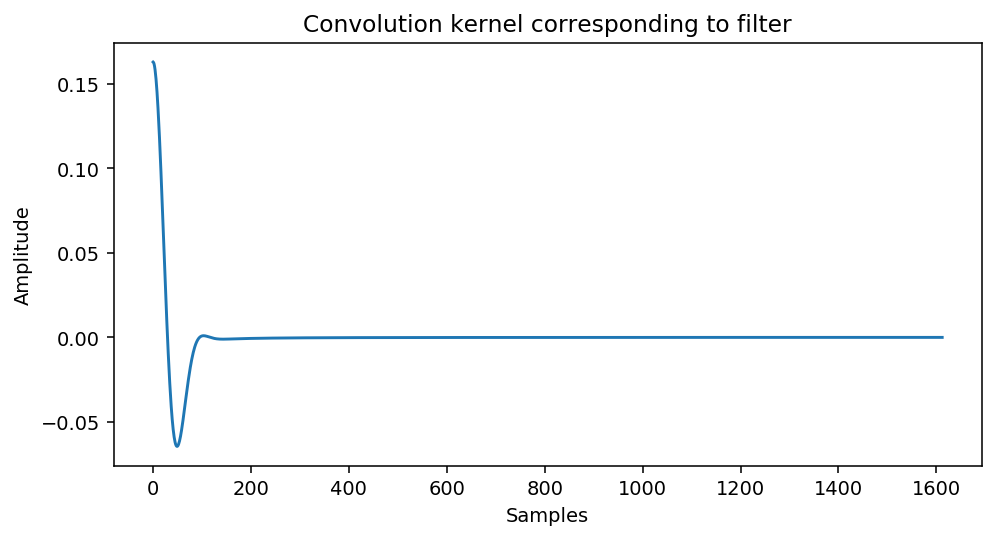
\includegraphics[scale=0.6]{src/6.29 sunspots convolution kernel.png}
    \caption{The convolution kernel of the filter.}
\end{figure}
\noindent We can apply the convolution to the original signal now to get a new signal.
\begin{figure}[H]
    \centering
    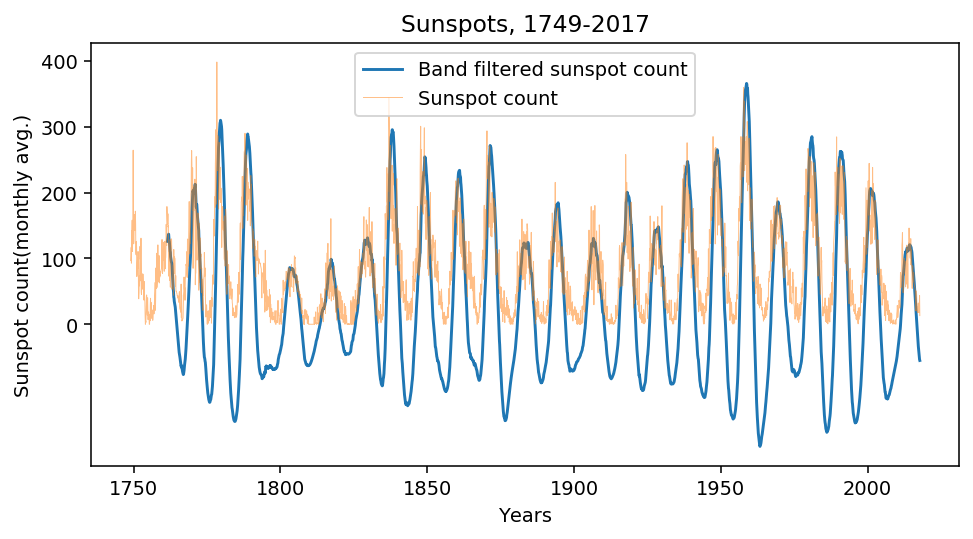
\includegraphics[scale=0.6]{src/6.30 sunspots convolved.png}
    \caption{The number of sunspots seen every 5 years, after convolving.}
\end{figure}
\noindent We can also look at this filtered signal in the frequency domain again, and see how the frequencies have been changed by applying the convolution kernel to the signal.
\begin{figure}[H]
    \centering
    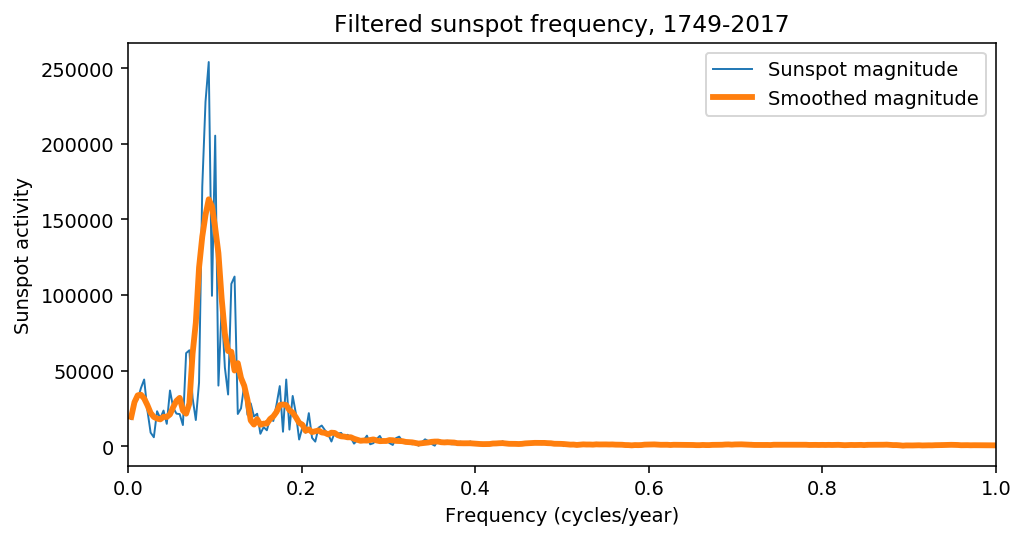
\includegraphics[scale=0.6]{src/6.31 sunspots convolved frequency.png}
    \caption{The DFT of the convolved signal.}
\end{figure}
\noindent The frequency of interest (0.1) has been preserved and the remaining frequencies have been dampened, as we had designed it.

\end{document}
